\subsection{Saturday Morning Setup}

The \pbproleref{role:primary_promoter} should plan to be the first person at the race, arriving at least two hours before the first race of the day
(\reffig{early_am_setup}).

\begin{marginfigure}
  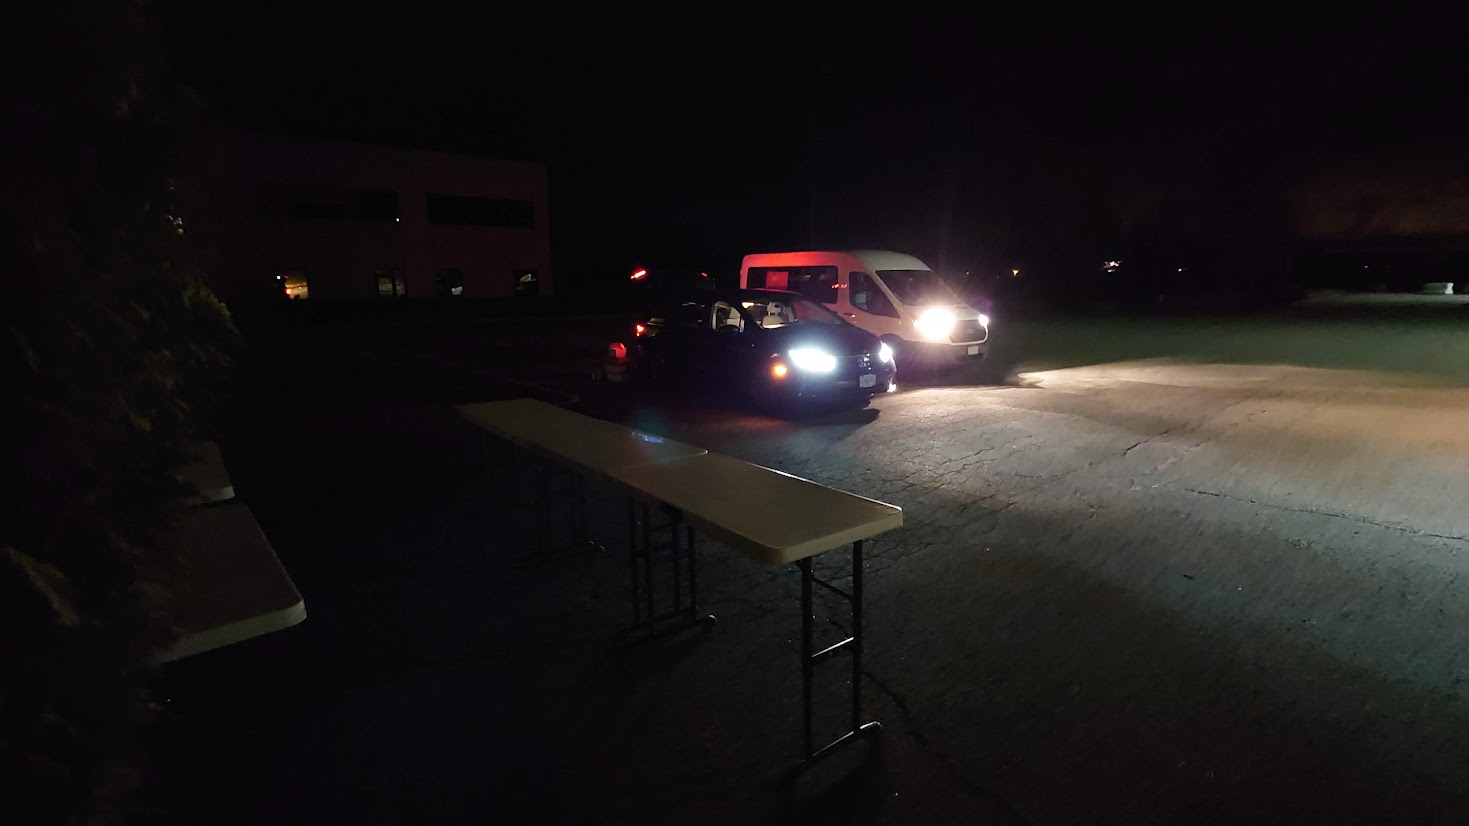
\includegraphics{2022_umass_early_am.jpg}
  \caption[Early morning race setup]{Expect to be setting up well before sunrise.\\
            Credit: Flyyn Leonard}
  \labfig{early_am_setup}
\end{marginfigure}

The \pbproleref{role:primary_promoter} should use this time to do a final check of the course,
ensuring that there are no hazards (sand on course, etc),
and that all directional signs and barriers are ready for the race.

If a location for the finish line has not been finalized, the \pbproleref{role:primary_promoter} should finalize that location now,
so the timing company, race officials, and riders can be informed of its location.

The \pbproleref{role:registrar} and \pbproleref{role:secondary_promoter} should be the next to arrive, at least 90 minutes before the first race of the day.

\subsubsection{Registration Setup}

The \pbproleref{role:registrar} should start setting up registration with assistance from the \pbproleref{role:primary_promoter} or \pbproleref{role:secondary_promoter}.

Registration must open 1 hour before the first race of the day, so setup is typically a high priority to ensure everything is ready before participants arrive.

\begin{itemize}
  \item Setup cover for registration - either hold registration inside or under the branded ECCC pop-up tent
  \item Ensure registration is locatable. If registration is under the branded ECCC tent that is typically sufficient, but if buildings block the view,
    ensure signs guide participants to registration
  \item Setup tables - typically a line of tables that participants approach, and additional tables at the back of the registration space
  \item Setup power
  \item Setup computers, printers, printers, the cash box
  \item Prepare supplies so they are easy to access: bib numbers, blank waivers, somewhere to store completed paperwork
\end{itemize}

\subsubsection{Volunteer Arrival}

The \pbproleref{role:volunteer_coordinator} should ask that the first set of volunteers arrive between 60-90 minutes before the first race starts -
not so early that the volunteers disrupt the registration setup and first course sweep, but not too late that they need to be given directions
within the hectic hour before the first race.

\subsubsection{T-60 Minutes}

While the earlier hours are typically dark and quiet, everything starts to get busy one hour before the first race of the day starts.

Participants will start arriving in large numbers, needing help parking and directions to registration.
The \pbproleref{role:registrar} and any registration assistants will have their hands full processing registrations and handing out bib numbers,
and also being the point person that everyone asks for the day's schedule, which side to pin numbers on, and for directions to the bathrooms.

\begin{marginfigure}
  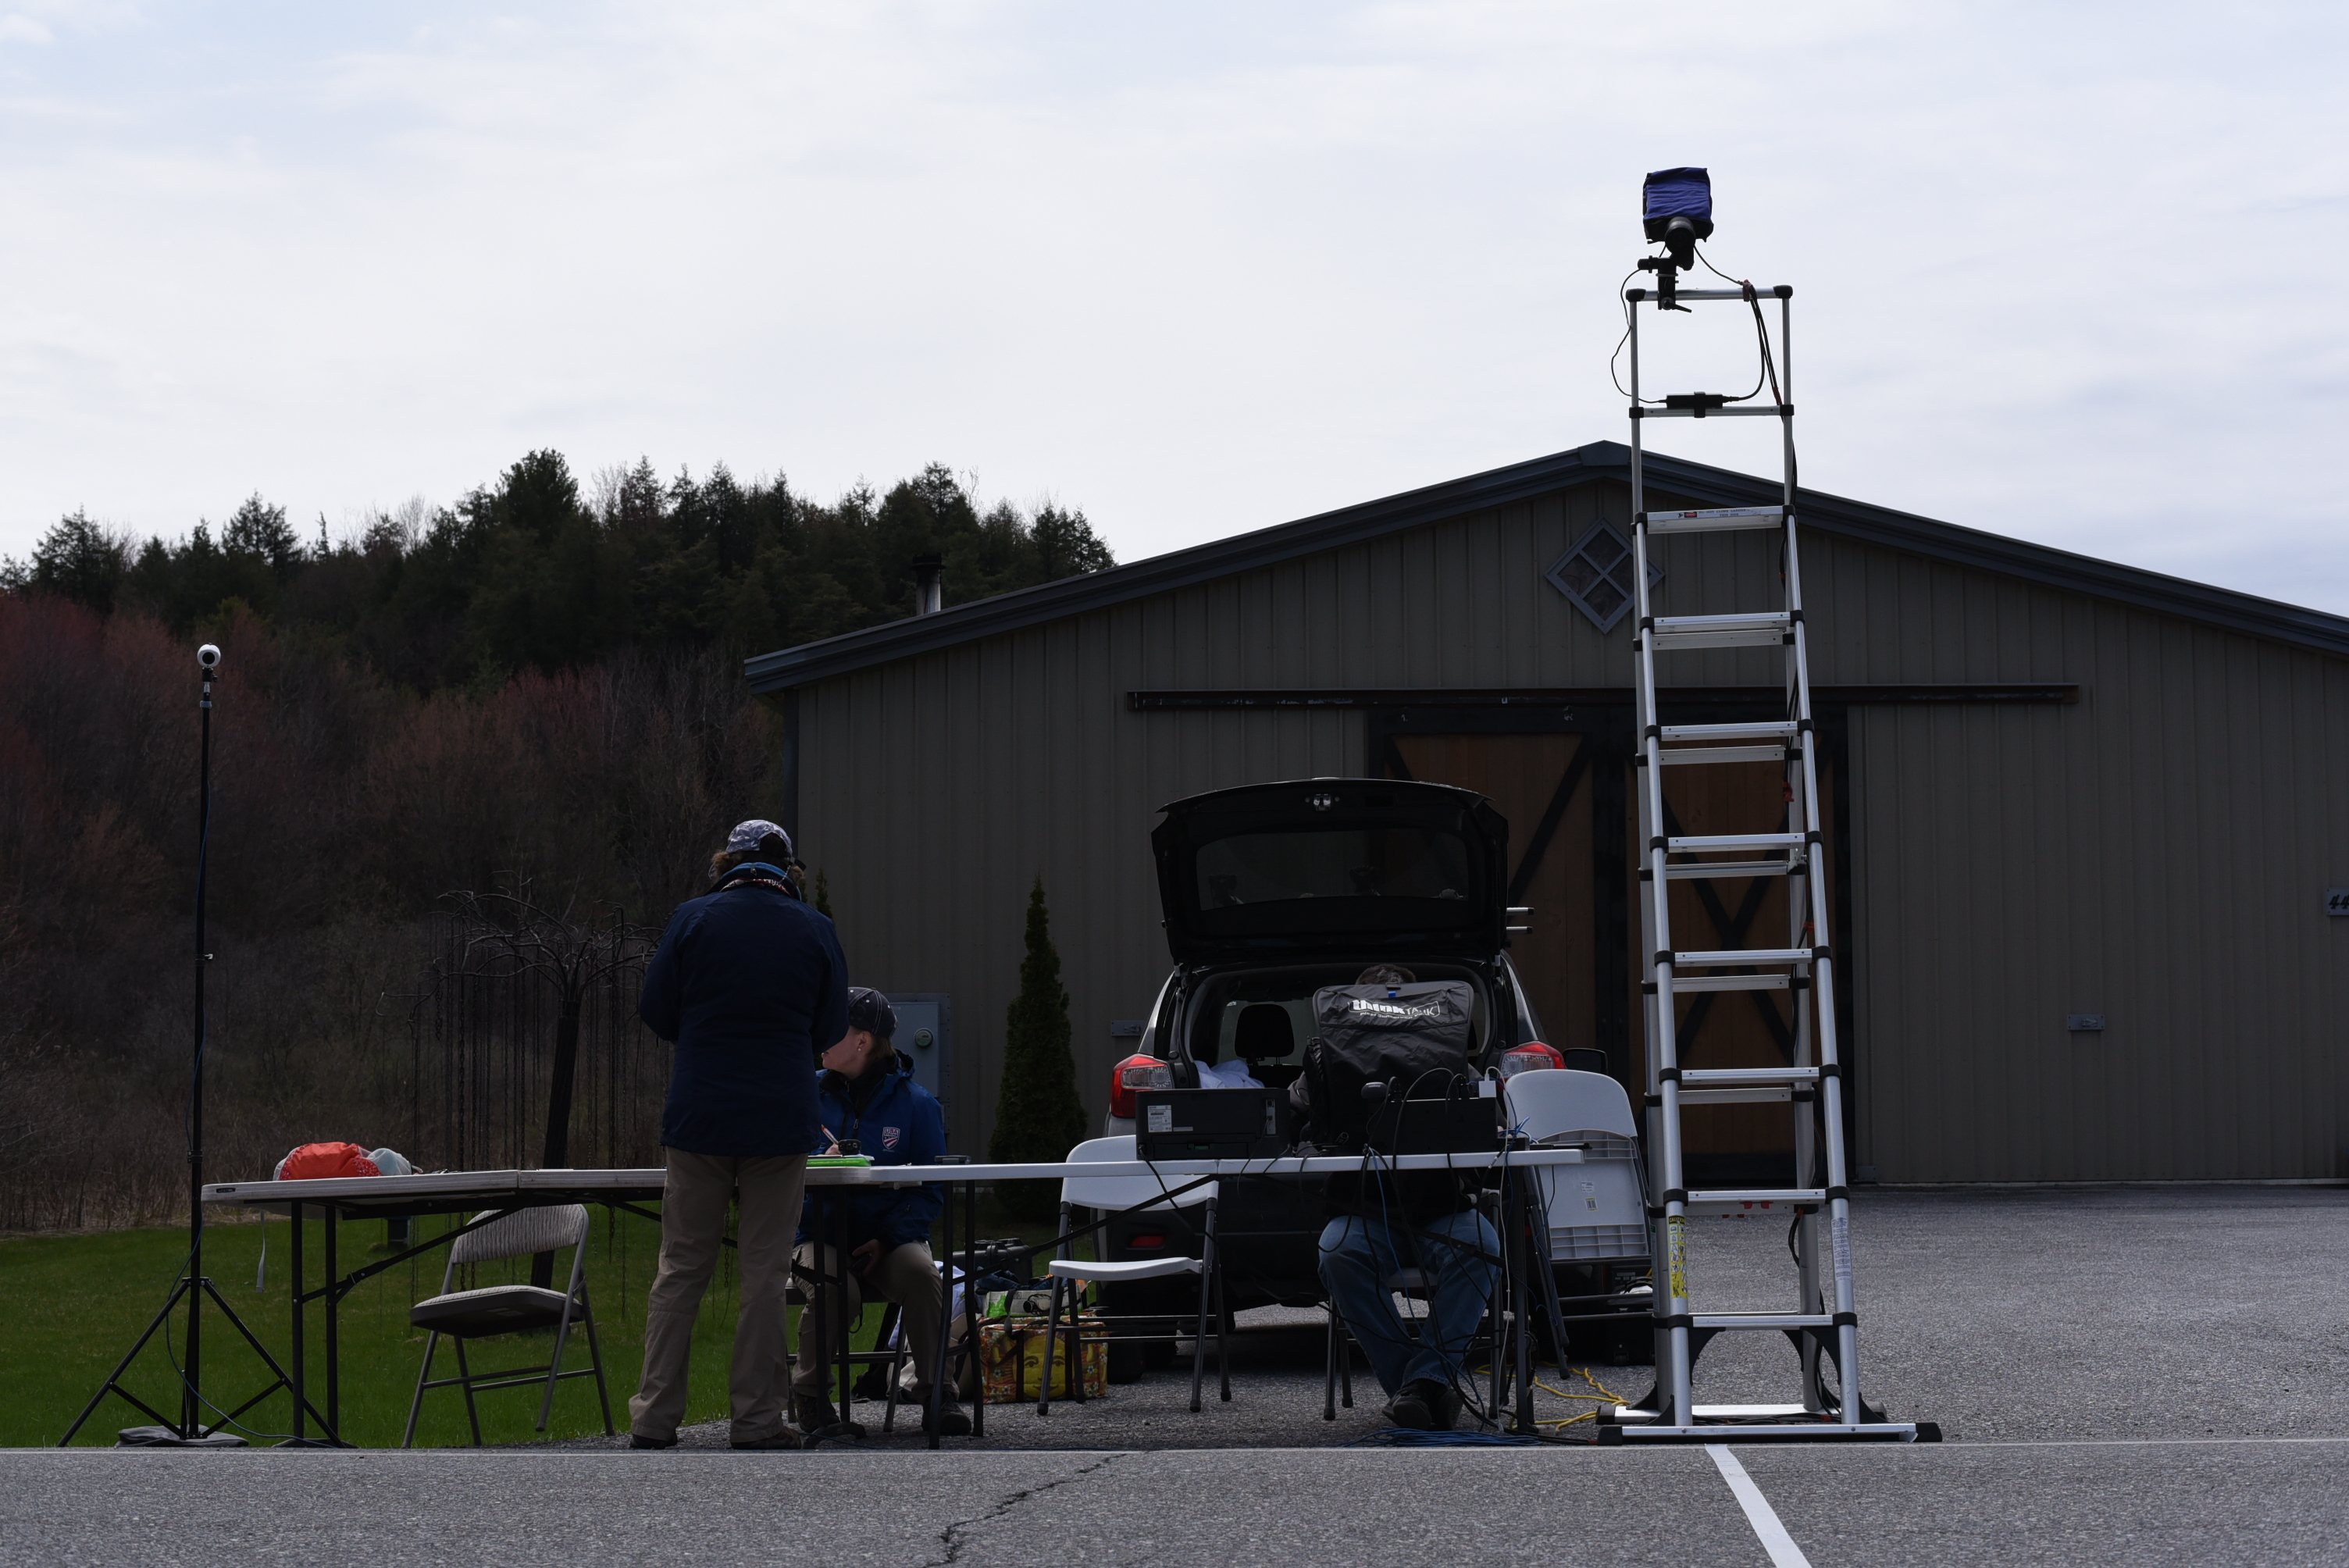
\includegraphics{2022_uvm_finish_line.jpg}
  \caption[A finish line setup with equipment, timing company, and USA Cycling officials]{The finish line at the 2022 UVM Race with timing equipment run by an independent timing company and
            USA Cycling officials.\\
            Credit: Bucknell Cycling}
  \labfig{pbp_road_finish_line_setup}
\end{marginfigure}

The timing company should arrive at least one hour before the first race.
The \pbproleref{role:primary_promoter} should greet them when they arrive,
and show them where the finish line is so the timing company can setup their equipment (see \reffig{pbp_road_finish_line_setup} for an example setup).

\index{officiating}
Race officials should be told to arrive one hour before the first race starts%
\sidenote{This is a USA Cycling standard.}.
The \pbproleref{role:primary_promoter} should meet the USA Cycling officials when they arrive.
The officials should be shown where everything is located, and the promoters should attend a briefing with the officials,
and ensure everyone is on the same page regarding communication (especially ensuring that race staff are not using a radio channel that the officials think is officials-only).

\subsubsection{T-30 Minutes}

Medical standby/EMTs should arrive around 30 minutes before the first race.
The \pbproleref{role:secondary_promoter} should meet them when they arrive,
providing them with communication methods (radios, cell phone numbers), maps, and brief them on what the day will entail.

Police detail officers should also be arriving around 30 minutes before the first race.
The \pbproleref{role:secondary_promoter} should meet and brief the officers, and ensure the officers block roads with barriers
before the race begins.

If the criterium is using a lead car, the \pbproleref{role:assistant_promoter} and Volunteer Coordinator should ensure the vehicle and driver are ready.
The \pbproleref{role:secondary_promoter} should tape a "Lead Car" sign to the front and rear windows,
give the driver a radio and a short briefing.

\subsubsection{T-20 Minutes}
\labsubsec{road_pbp_crit_t-20}

Before getting the first race lined up, the \pbproleref{role:primary_promoter} should check that everything is ready:

\begin{itemize}
  \item Are all roads closed, with proper police details and marshals ensuring a safe race?
  \item Are all hazards clear, including:
  \begin{itemize}
    \item No cars on course in dangerous locations
    \item Any dangerous potholes or sewer grates are covered
    \item Potential crash points, including telephone poles, cars, and fences are covered with hay bales or another crash barrier
  \end{itemize}
  \item Is the finish line setup and are the Timing Company and \pbproleref{role:chief_judge} ready?
  \item Is the \pbproleref{role:chief_ref} ready to start the race?
  \item Is Medical Standby ready and on-duty, and properly briefed?
  \item Did the majority of students have some issue getting to the race and registering?
\end{itemize}

If any of the above items are not ready, the \pbproleref{role:primary_promoter} should determine if races should be delayed.
If a delay is appropriate, it should be announced to all riders.

The \pbproleref{role:secondary_promoter} should work with the \pbproleref{role:volunteer_coordinator} to deploy any marshals who have not already gone out,
ensuring all marshals have a safety vest, radio, and have been briefed.
